
\documentclass{beamer}
\usepackage[orientation=portrait, size=a1, scale=1.4, debug]{beamerposter}
\usetheme{unn}

\usepackage{cmbright}

\usepackage{fontspec}

\setmainfont{Times New Roman}
\setromanfont{Times New Roman}
\setsansfont{Times New Roman}

\usepackage{polyglossia}
\setmainlanguage{russian}
\usepackage{csquotes}

\usepackage{booktabs}
\usepackage{ragged2e}

\usepackage[backend=biber,
            movenames=false,
            maxnames=4,
            style=gost-numeric,
            sorting=nty,
            autolang=other]{biblatex}
						
%\newfontfamily\cyrillicfonttt{lmmonolt10-regular.otf}
%\newfontfamily\cyrillicfontsf{lmsans10-regular.otf}						
					
\addbibresource{bibliography.bib}

\DeclareMathOperator{\re}{\operatorname{Re}}

\title{Решение многомерных задач глобальной оптимизации с использованием Intel oneAPI }
\author{К.А. Баркалов \and И.Г. Лебедев \and Я.В. Кольтюшкина}
\institute{Нижегородский государственный университет им. Н.И. Лобачевского}
\setlength{\abovedisplayskip}{3pt}
\setlength{\belowdisplayskip}{3pt}

\begin{document}
\begin{frame}[t]
    \begin{columns}[t]
        \begin{column}[t]{0.48\paperwidth}
            \begin{block}{Постановка задачи}
             Задача многомерной многоэкстремальной оптимизации может быть определена как поиск наименьшего значения действительной функции \(\phi(y)\)  в гиперинтервале \(D=\{y\in R^N:a_i\leqslant x_i\leqslant{b_i}, 1\leqslant{i}\leqslant{N}\}\). 
Будем предполагать, что целевая функция задана как <<черный ящик>> и удовлетворяет условию Липшица с априори неизвестной константой \(L\)

          \end{block}
          
          \begin{block}{Редукция размерности с помощью кривых Пеано}

В ННГУ им. Н.И. Лобачевского под руководством проф. Р.Г. Стронгина разработан эффективный подход к решению задач глобальной оптимизации \cite{Strongin2013}. В рамках данного подхода решение многомерной задачи сводится к решению эквивалентной ей одномерной задачи. Для этого используется редукция размерности с помощью кривой Пеано \(y(x)\), которая непрерывно и однозначно отображает отрезок вещественной оси \([0,1]\) на \(N\)-мерный куб \cite{Sergeyev2013}.

 \begin{minipage}[t]{.48\textwidth}
              \begin{figure}
                  \centering
                  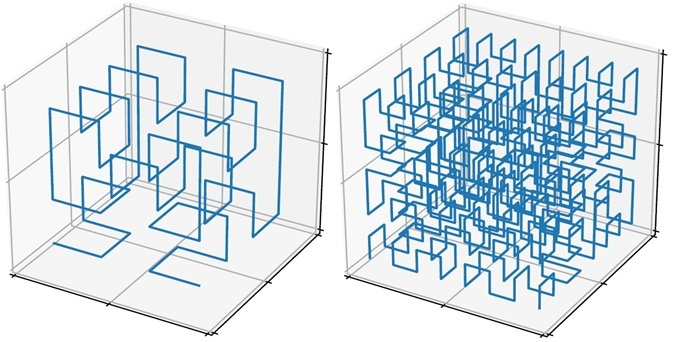
\includegraphics[scale=1.27]{images/pean_2.jpg}
              \end{figure}
              \end{minipage}
              


\end{block}
\begin{block}{Метод глобальной оптимизации}

В процессе работы алгоритма строится последовательность точек \(x^k\), в которых проводятся \textit{испытания}, т.е. вычисляются значения целевой функции \(\phi^k=\phi(y(x^k))\). 

Общая схема одной итерации одномерного метода:
              \begin{enumerate}
                \justifying
                \item Упорядочить точки предшествующих испытаний в порядке возрастания их координат: \(a=x_{0}<...<x_{i}<...<x_{k}=b\).
                \item Вычислить для каждого интервала \((x_{i-1};x_{i}),1\leq i\leq k\)  характеристику \(R(i)\) .
                \item Определить интервал \((x_{t-1};x_{t})\) , которому соответствует максимальная характеристика \(R(t)=\max\{R(i),1\leq i\leq k\}\).
                \item Провести следующее испытание в точке \(x^{k+1}=d(t)\in (x_{t-1};x_{t})\) , где \(d(t)\)  — правило размещения точки следующего испытания в интервале с номером \(t\).
                \item Проверить выполнение критерия остановки \(x_{t}-x_{t-1}<\varepsilon\).
              \end{enumerate}

 \begin{minipage}[t]{.48\textwidth}
              \begin{figure}
                  \centering
                  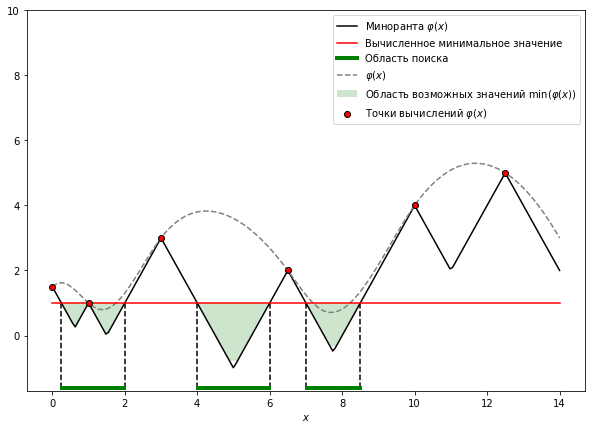
\includegraphics[scale=1.27]{images/PlotGS.png}
              \end{figure}
              \end{minipage}
\end{block}
            
        \end{column}
        \begin{column}[t]{0.48\paperwidth}
          \begin{block}{Организация распараллеливания}

Распараллеливание организовано следующим образом: в ходе выполнения одной итерации алгоритма одновременно проводятся \(P \geq 1\) испытаний в различных точках области поиска. Важно отметить, что рассматриваются функции, в которых самым трудоемким и времязатратным этапом работы является это вычисление значения функции в точке. Поэтому организация одновременных вычислений этих значений положительно влияет на скорость работы алгоритма для таких функций. 


\end{block}

\begin{block}{Использование Intel oneAPI}

Одним из вариантов реализации данного подхода является использование набора инструментов Intel oneAPI. Достоинством Intel oneAPI является простота, открытость и возможность легкой интегрирации в существующий код. Intel oneAPI позволяет написать код один раз и в дальнейшем запускать его на различных устройствах. 

В рамках данной задачи нам необходимы возможности распараллеливания, которые обеспечиваются за счет включения в oneAPI языка data parallel c++ и набора библиотек, облегчающих межархитектурную разработку.  


\end{block}
%----------------------------------------------------------------------------------------
%	RESULTS
%----------------------------------------------------------------------------------------

\begin{block}{Результаты}

На данный момент получены результаты вычислительных экспериментов, в которых тестовые задачи формируются специальным генератором \cite{GKLS}. В таблицах \ref{table:GKLS_RES_1}, \ref{table:GKLS_RES_2} приведены среднее число итераций параллельного алгоритма глобального поиска и ускорение относительно последовательной версии. В каждом эксперименте решалось 100 задач размерности \(N = 4\) и \(N = 5\). Эксперименты проведены на компьютере с процессором Intel Core I5-7300HQ 2.5 GHz с видеокартой HD Graphics 630, 16 GB RAM, использовался язык \textit{data parallel c++}.



\begin{table}[!hbp]
    \centering
    \caption{Число итераций и ускорение при решении серии задач размерности $N=4$}
    \begin{tabular}{|c|c|c|}
    \hline
    P    & Итерации ($N=4$) & Ускорение ($N=4$) \\ \hline
	128 & 106.5   & 4.7    \\ \hline
	256 & 41.3    & 8.5          \\ \hline
	\end{tabular}
    
    \label{table:GKLS_RES_1}
\end{table}

\begin{table}[!hbp]
    \centering
    \caption{Число итераций и ускорение при решении серии задач размерности $N=5$}
    \begin{tabular}{|c|c|c|}
    \hline
    P    &         Итерации ($N=5$) & Ускорение ($N=5$) \\ \hline
	128 &        235.6   & 4.4      \\ \hline
	256 &       90.5    & 9.2      \\ \hline
	\end{tabular}
    
    \label{table:GKLS_RES_2}
\end{table}
     
\end{block}
          \begin{block}{Литература}
            \printbibliography
            
          \end{block}
        \end{column}
    \end{columns}
\end{frame}
\end{document}


